\subsection{Methodological Literature}

Based on the systematic review and its coding, the first data set we
assess is a database of scale validations. We bring together the scales
suggested in previous reviews as well as validation studies we
identified in our own review. Throughout our literature review we found
five major works that reviewed the measurement of acculturation
\citep{Celenk2011, Maestas2000, Matsudaira2006, Wallace2010, Zane2004}.
After the removal of duplicate scales, we added any scale validation
that was present in our own systematic review but not included in the
previous reviews. For each measure we extracted the full item list as
well as the item scoring prior to coding. A comprehensive and
interactive database of the scales, with reference- and publication
information, as well as our experience elements and -context coding is
available in our online supplementary information as well as on our open
science repository (\hl{OSF and/or github citation here}).

\subsubsection{Methods}

Taken together these five reviews collected a total of 197 scales, of
which 75 were duplicates. From our own review we added 25 additional
validation studies. After removing duplicates this meant that we
considered a total of 122 unique scales for our coding. Of these scales
we ultimately had to exclude 41, because they were either not accessible
or did not fit the the topic of our review (see Table
\ref{tab:ScalesExclusion}). The scales had an average of \hl{X.XX} items
and \hl{X.XX} sub-scales. Most items were rated on a five-point
(\hl{XX.XX}\%) or four-point likert-type scale (\hl{XX.XX}\%), with only
\hl{X} scales including categorical ratings. About a fifth of scales
(20.4918\%) included majority group members in their validation studies.
The earliest included validation was from 1972 with a majority of scales
being validated around the turn of the 21\textsuperscript{st} century
and the latest included validation study in 2018.

\begin{table}

\caption{(\#tab:ScalesExclusion)Reasons for Exclusion}
\begin{tabular}[t]{lc}
\toprule
Exclusion Reason & Frequency\\
\midrule
not migration & 14\\
items not included & 8\\
search pending & 5\\
not accessible & 4\\
not found & 3\\
not acculturation & 2\\
majority focussed & 1\\
not found probably the same as Tsai et al. 2000 & 1\\
only language (no scale) & 1\\
same as S-029 & 1\\
uses other scale & 1\\
\bottomrule
\end{tabular}
\end{table}


\subsubsection{Results}

For the literature on scale validations, we assessed both the role of
experience elements in the measures as well as contextual differences.

\paragraph{Experience}

With our main aim of examining the experience structure within the
scales, we examined whether scales included a specific experience
elements but also examined the used elements in their complex
combinations. In terms of general inclusion of elements, most studies
included a measure of cognition (89.66\%) and behavior (82.76\%),
whereas only roughly half the studies included a measure of affect
(55.17\%) and only a fourth of the scales included a measure of motives
(28.74\%). However, only a minority of scales included only a single
dimension. There were only 5 scales that exclusively relied on
cognitions (5.75\%) and 4 scales that measured only behaviors (4.6\%).
Yet, inversely, there were also only 13 scales that measured all four
dimensions (14.94\%). Most studies measured two (37.93\%) or three
(36.78\%) dimensions. A majority of scales either measured behavioral
and cognitive elements (26.44\%) or behavioral, cognitive, and affective
elements (26.44\%; also see Figure \ref{fig:ElementsScales} and Table
\ref{tab:ScaleElementCooccurrences}). Looking at the number of elements
measured together we also see substantial differences in what kind of
scales include a certain element. Scales that included cognitions
measured an average of 2.67 elements, scales measuring behavior, on
average, measured a 2.71, while scales that included affect measures had
a complexity average of 3.1 and scales measuring motivation even
measured an average of 3.4 scales. Thus, most scales measure multiple
dimensions, yet they focus on easily accessible dimensions (i.e.,
behavior and cognition), less of what is considered `less accessible' or
`subjective' (i.e., affect and desires). This is also visible in the
circumstance that there were no scales that exclusively measured
motivational or emotional adaptation (while this was the case for both
cognitions and behaviors). And if emotional or motivational aspects were
measured they were on average measured in scales that were already more
complex (i.e., included more experience elements).

\begin{figure}[h]
\centering
\caption{Scales: Bar graph of the experience element combinations.}
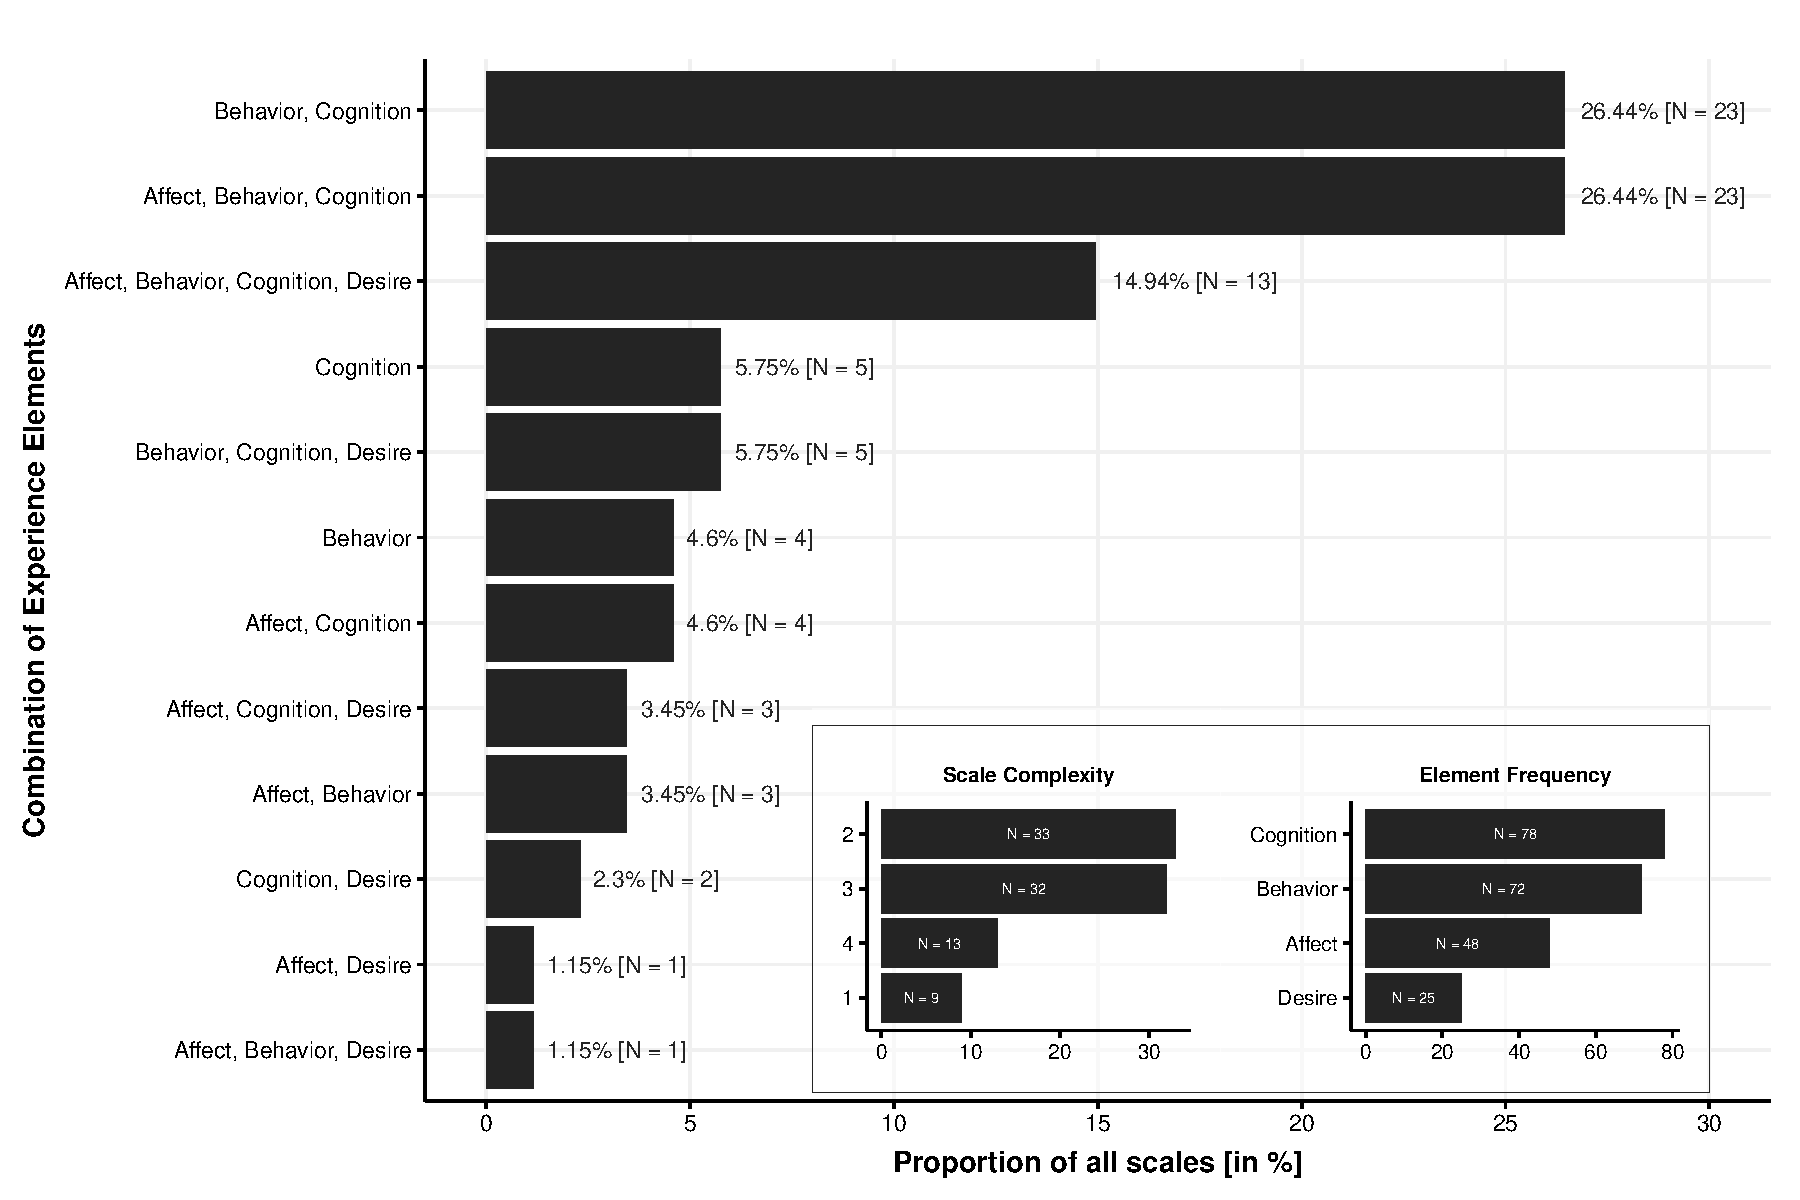
\includegraphics[width=\textwidth]{Figures/ABCDFreq-1}
\label{fig:ElementsScales}
\end{figure}

\begin{table}

\caption{\label{tab:ScaleElementCooccurrences}Scales: Element Co-occurrence Matrix}
\begin{tabular}[t]{lcccc}
\toprule
  & Affect & Behavior & Cognition & Desire\\
\midrule
Affect & 48 & 40 & 43 & 18\\
Behavior & 40 & 72 & 64 & 19\\
Cognition & 43 & 64 & 78 & 23\\
Desire & 18 & 19 & 23 & 25\\
\bottomrule
\end{tabular}
\end{table}

\paragraph{Context}

To gain a general understanding of contextual factors within the
validated studies, we also assessed cross-study patterns of cultural,
individual, situational, and process-related focus points.

\subparagraph{Country}

To assess the cultural contexts for which scales were validated we
assessed the migrants' countries of settlement as well as the countries
of origin. We found that most scales investigated a single host country
(\textit{N} = 81) and most investigated one country of origin
(\textit{N} = 68). There was 1 scale that was validated in two countries
and 1 that was validated in three countries. Additionally, there was a
single scale that was validated in a larger multi-national survey
context (i.e., with multiple host and origin countries). There was also
one study with two scales that were validated with the origin culture as
the starting point (i.e., single origin country, multiple host
countries). Looking at the country patterns, we found that an
overwhelming number of scales were validated within a U.S. American
settlement context (\textit{N} = 61). But also the remaining receiving
societies were mostly `western' countries (e.g., Canada, The
Netherlands, The United Kingdom, Israel, Australia) with only individual
scales for Taiwanese, Nepalese, or Russian settlement contexts. For the
migrant origin societies there was slightly more variation. There were a
few migrant groups that were investigated specifically (e.g., Mexico:
14, China:7, South Korea: 4), however most validation studies targeted
broader categories of migrants (any migrants: 11, Asian: 5, Hispanic: 9,
LatinX: 5). This also made it difficult to identify patterns of cultural
combinations investigated (apart from Mexican and LatinX migrants in the
United States).

\subparagraph{Sample}

To assess the role different groups of individuals targeted in the scale
validations, we coded the types of samples recruited for the validation
studies. A majority of studies sampled any consenting adult from the
migrant group of interest (\textit{N} = 50). As seems common in academic
research, a larger portion of the validated scales relied on young
migrants or students (\textit{N} = 29). Interestingly, only small
minority of validated scales targeted more vulnerable groups, such as
clinical samples (\textit{N} = 2) or refugees (\textit{N} = 2) --
despite a considerable focus on these groups within the broader
literature.

\subparagraph{Domains}

To assess the situational focus within the validated scales, we assessed
the number of domains within each scale as well as more common domains
across the scales. A relatively large number of scales asked about the
current state of the migrant in general manner without mentioning any
context or life domain (\textit{N} = 24; e.g., `'In general, in what
language do you read and speak?'`). The remaining scales referred to an
average of 3.49 dimensions (\textit{SD} = 3.42, range: 1 -- 21). A total
of 179 unique domains was measured across the 87 scales. The domains of
'language` (\hl{XX}\%), 'food' (\hl{XX}\%), `interactions' (\hl{XX}\%),
`family' (\hl{XX}\%) and `values' (\hl{XX}\%) were focused on most often
(see Online Supplementary Materials \hl{X}, Figure \hl{X}). Thus, while
there was large variation between the scales in the number, and
diversity of domains, the most frequently mentioned domains were in line
with the life domains proposed in the literature
\citep[e.g.,][]{Arends-Toth2007}.

\vspace{1em}
\todo[inline]{Should be re-coded to test our proposed domains. Also, re-check `general' code}

\subparagraph{Migration time}

All scales were validated using cross-sectional data after the migrant
arrived in the settlement society. This is in line with observations by
previous reviews of the field \citep[e.g.,][]{Brown2011}.

\subsection{Empirical Literature}

After analysis of the scales validations, we assessed the broader
empirical works we collected within the systematic review. We first
looked at all available empirical publications (incl.~books, chapters,
and dissertations). We later also assessed differences between fields
the work was published in. However, because we considered the fields on
an audience level, we used only empirical journal articles -- for which
journal-level audience data is available.

\subsubsection{Methods}

The search produced a total of \hl{XXX} results to which we added
\hl{XX} articles through contacts with experts in the field. We
subsequently screened out results that did not fit into our review.
After duplicate removal (\(N_{excluded}\) = \hl{XX}, \(N_{screened}\) =
484), we excluded 92 results in the title screening as well as an
additional 126 results during the abstract screening. Of the remaining
266 results, 259 papers presented empirical work on acculturation and
were coded. The 7 non-empirical results were reviews, which were not
coded because they did not fit into our coding schema. During the full
text coding we excluded an additional 26 results because they were
either not relevant or were not accessible (for exclusion reasons see
Table \ref{tab:EmpiricalExclusion} and for our PRISMA diagram see Figure
\ref{fig:PRISMA}).

\begin{figure}[h]
\centering
\caption{PRISMA diagram. Position still undecided. Currently generated in R based on n(row) maybe make prettier. \Warning\ Re-check numbers before duplicates removed and number of papers added from other sources.}
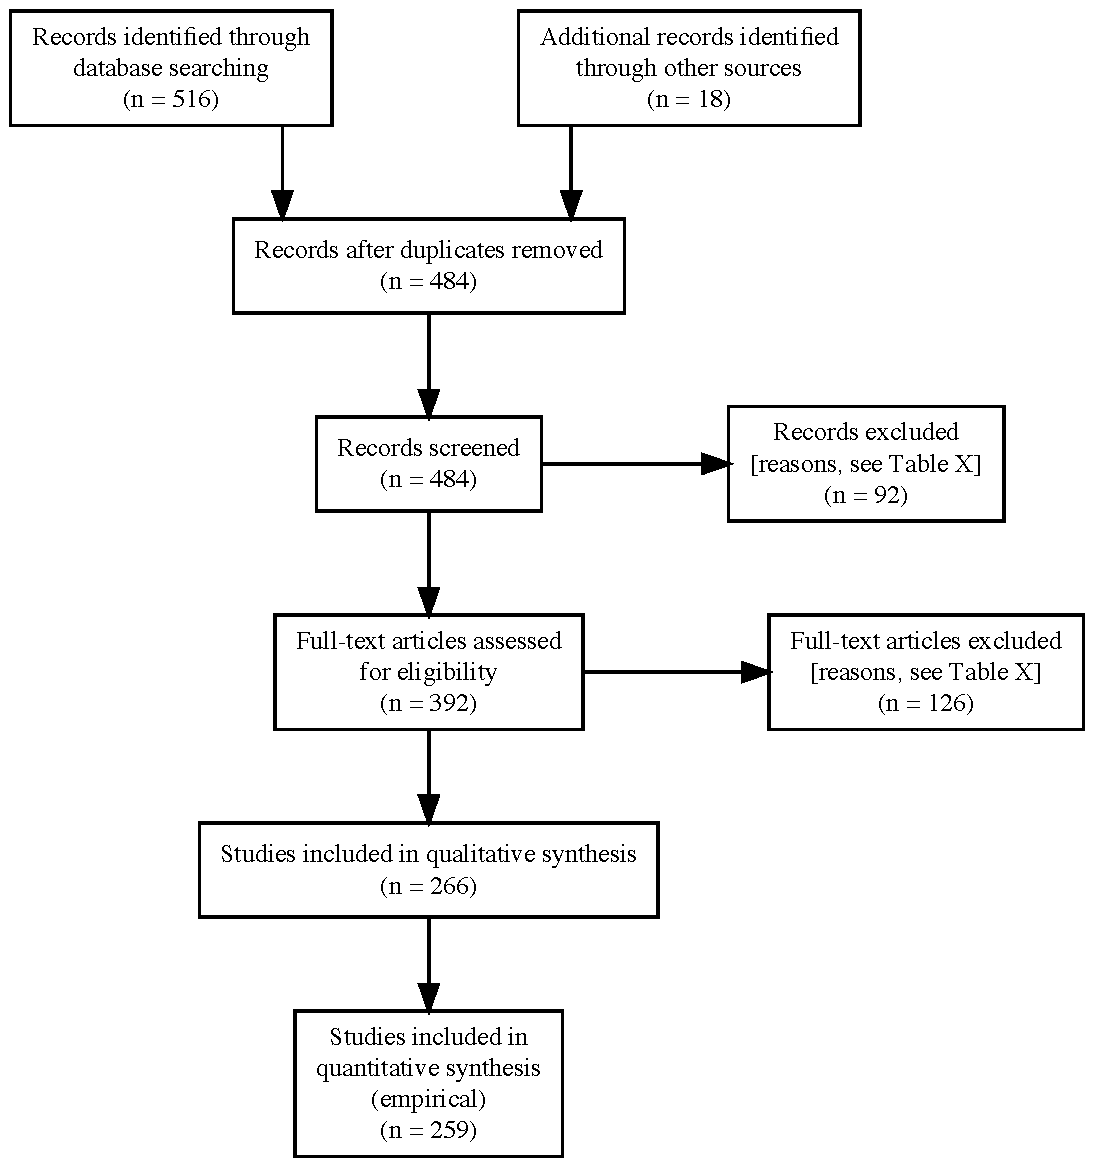
\includegraphics[width=\textwidth]{Figures/PRISMA}
\label{fig:PRISMA}
\end{figure}

\begin{table}

\caption{\label{tab:EmpiricalExclusion}Exclusion Reasons Empirical Literature}
\centering
\begin{tabular}[t]{lccc}
\toprule
\multicolumn{1}{c}{ } & \multicolumn{3}{c}{Screening} \\
\cmidrule(l{3pt}r{3pt}){2-4}
Exclusion Reason & Title & Abstract & Full Text\\
\midrule
not migration & 36 & 27 & \\
not acculturation & 19 & 49 & \\
not experience & 19 & 24 & \\
not migrant & 17 & 18 & \\
not measured &  & 8 & 2\\
re-migration &  & 1 & \\
thesis not accessible &  &  & 13\\
book not accessible &  &  & 4\\
items not accessible &  &  & 4\\
article not accessible &  &  & 2\\
should still be coded &  &  & 1\\
\bottomrule
\end{tabular}
\end{table}


Of the final works we coded, 192 were journal articles, 37 theses, and 4
book chapters. Most studies presented quantitative data (\textit{N} =
205), mixed methods (\textit{N} = 14), or qualitative data (\textit{N} =
11), while the remaining 3 manuscripts were reviews of empirical data. A
vast majority of the authors used the term `acculturation' (or
derivative versions, such as `acculturation attitudes' or `acculturation
orientation'; \textit{total N} = 178), or `integration' (\textit{N} = 7)
to refer to cultural adaptation. Notably, a majority of the empirical
investigations did not share common measures of cultural adaptation --
186 studies used measures that were reported a maximum of five times,
with a considerable majority of papers using new or ad-hoc measures of
cultural adaptation. Only about every tenth study included the local
majority in the study (\textit{N} = 25, 10.8225\%). Cultural adaptation
most frequently was a predictor variable (\textit{N} = 99, 42.8571\%), a
dependent variable (\textit{N} = 72, 31.1688\%), or a correlation
variable (\textit{N} = 27, 11.6883\%) in the empirical works. This
pattern was mirrored when looking at the focus of the papers, where a
majority of the papers had acculturation as their main focus (\textit{N}
= 83, 36.7257\%), with other bodies of work focusing on health outcomes
(\textit{N} = 23, 10.177\%), or inter-group relations (\textit{N} = 12,
\texttt{empFocusRelationPerc}\%) as their main outcomes. The earliest
included study was published in 1970, with a continuous increase of
publications after the year 2000, with considerable publication peaks in
2011 and 2019. We provide full descriptions of descriptive data
extractions and additional information about the data description in
Online Supplementary Information X.

\paragraph{Field of Publication}

For the broader empirical literature, we also collected additional data
on the field the studies were published in. To assess the differences
between fields we merged the `Scimago Journal Ranking Database'
\citep{SCImago2020} with our empirical review. For all available journal
articles we added information on key journal metrics (incl.~H index,
impact factor, and data on the field and audiences). This also meant
that dissertations, book chapters, and books were excluded from this
analysis because data on their publishers is not readily available or
unreliable. Additionally, 8 journals were not included in the Scimago
database (likely because they do not have an ISSN identifier or were
discontinued before 1996, see Online Appendix \hl{X}, Table \hl{X} for
the missing journals). We ultimately had journal metrics for 183
empirical articles. The Scimago database classifies each journal
according to the field(s) that the journal aims to address. Importantly,
(1) each journal can be be classified to address multiple fields and (2)
the field include codes of fields (e.g., `Social Sciences') as well as
sub-fields (e.g., `Social Psychology'). This leads to the case that
there can be substantial overlap between fields, and journals cannot
easily or readily be assessed in mutually exclusive subgroups.

To summarize the articles further we then classified the field
combinations into super-ordinate discipline codes. These discipline
codes are based in part on U.S. Department of Education's subject
classifications \citep[i.e., CIP;][]{InstituteofEducationSciences2020},
the U.K. academic coding system
\citep[JACS 3.0;][]{HigherEducationStatisticsAgency2013}, the Australian
and New Zealand Standard Research Classification
\citep[ANZSRC 2020;][]{AustralianBureauofStatistics2020}, as well as the
Fields of Knowledge project \citep{ThingsmadeThinkable2014}. We
ultimately classified each journal into one of four mutually exclusive
disciplines (psychology: \textit{N} = 61, multidisciplinary: \textit{N}
= 57, Medicine, Nursing, and Health: \textit{N} = 51, and Social
Sciences (miscellaneous): \textit{N} = 14. For a full discussion of the
classifications see Online Supplementary Materials \hl{X}).

\subsubsection{Results}

To test the utility of our framework, we again assessed the role of
experience elements in the measurement as well as contextual
differences.

\paragraph{Experience}

In terms of the overall frequencies of experience elements, the broader
empirical data mirrored that of the validation studies. Most studies
included a measure of cognition (83.26\%) and behavior (80.69\%),
whereas only about half of all studies included a measure of affect
(51.93\%) and only a fifth of the studies included a measure of motives
(18.45\%). Yet, only 42 studies focused on a single element
(\(N_{behavior\ only}\) = 20, \(N_{cognition\ only}\) = 18,
\(N_{emotion\ only}\) = 4). Similarly, only 17 papers included measures
of all four experience elements (7.3\%). Most studies measured three
(37.77\%) or two dimensions (36.91\%). Different from the scale
validations, within the broader empirical works most works included
measures of emotions, behaviors, and cognitions (\textit{N} = 69,
29.61\%), with a further substantial number of articles measuring
behaviors and cognitions (\textit{N} = 53, 22.75\%. Also see Figure
\ref{fig:EmpPlotFreq-1} and Table
\ref{tab:EmpiricalElementCooccurrences}). Looking at the number of
elements measured together we again see substantial differences in what
kind of scales include the individual elements. Scales that included
cognitions measured an average of 2.53 elements, scales measuring
behavior, on average, measured a 2.52, while scales that included affect
measures had a complexity average of 2.86 and scales measuring
motivation even measured an average of 3.23 scales. Thus, interestingly,
not a single study measured only motivation, and measures of motives
remained mostly limited to scales that were already multidimensional.
The results exacerbate the pattern found in the scale validations,
complex measures and conceptions of acculturation are seen infrequently
and readily accessible (i.e., less subjective) dimensions of cognition
and behavior remain the focus of most studies.

\begin{figure}[h]
\centering
\caption{Empirical Literature: Bar graph of the experience element combinations.}
\includegraphics[width=\textwidth]{Figures/EmpPlotFreq}
\label{fig:EmpPlotFreq-1}
\end{figure}

\begin{table}

\caption{\label{tab:EmpiricalElementCooccurrences}Empirical Literature: Element Co-occurrence Matrix}
\centering
\begin{tabular}[t]{lcccc}
\toprule
  & Affect & Behavior & Cognition & Desire\\
\midrule
Affect & 121 & 96 & 107 & 22\\
Behavior & 96 & 188 & 153 & 37\\
Cognition & 107 & 153 & 194 & 37\\
Desire & 22 & 37 & 37 & 43\\
\bottomrule
\end{tabular}
\end{table}


\paragraph{Context}

To gain a general understanding of contextual factors within the broader
empirical studies, we again assessed cross-study patterns of cultural,
individual, situational, and process-related focus points.

\subparagraph{Country}

To assess the cultural contexts on which the authors focused, we again
assessed the migrants' countries of settlement as well as the countries
of origin. Similar to the validations, an overwhelming number of scales
were validated within a North American settlement context (United
States: \textit{N} = 109, Canada: \textit{N} = 26). But also the
remaining receiving societies were mostly `western' -- Western Europe
(e.g., The Netherlands, United Kingdom, Germany, Italy, Spain),
Australasia (Australia, New Zealand), Russia, and Israel. And only 10
studies focused on data from multiple receiving societies.

When it came to the migrants' country of origin, a majority of studies
were indifferent to migrants background and simply recruited any
consenting migrant (\textit{N} = 37), or recruited a category of
migrants (e.g., LatinX or Hispanic: \textit{N} = 21, African: \textit{N}
= 10). Among the individual countries target there was a particular
focus on the east and south-east Asian region (e.g., China: \textit{N} =
21, South Korea: \textit{N} = 19, Vietnam: \textit{N} = 11). Yet,
different from the scale validations, there was a large variety of
different origin countries that were included in less than five studies
(\textit{N} = 101 regions were targeted less than five times). Thus, the
receiving countries mainly mirrored those for which scales were
validated, yet there was an extensive number origin countries which were
investigated individually or migrants were considered irrespective of
their cultural origin. Moreover, it was again not possible to identify
distinct cultural adaptation clusters within the literature (that would
be large enough to compare).

\subparagraph{Sample}

To assess the role different groups of individuals targeted in the
empirical work, we again coded the types of samples recruited for the
studies. A majority of studies sampled any consenting adult from the
migrant group of interest (\textit{N} = 145, 62.23\%). Of the targeted
sampling strategies, most recruited refugees (\textit{N} = 22, 9.44\%),
young migrants (\textit{N} = 20, 9.01\%), or elderly people (\textit{N}
= 14, 6.01\%). The remaining fifth of the studies recruited other more
specific samples (e.g., nurses, athletes, Muslims). Interestingly,
despite the circumstance that a large portion of papers focused on
mental health outcomes, only 7 studies (3\%) recruited clinical migrant
samples. These results speak to the case that relatively few empirical
studies actually take individual differences into account in their
sample selection. Studies may still address individual differences
within the data description and within the modeling approaches (e.g.,
controlling for gender), yet it seems that inter-sectional
idiosyncrasies did not seem to play a major role in the targeting of
samples.

\subparagraph{Domains}

To capture the situational focus of the authors, we coded which life
domains the utilized measures referred to. A relatively large number of
studies assess cultural adaption in general manner without mentioning
any context or life domain (\textit{N} = 116). The remaining studies
referred to an average of 2.16 dimensions (\textit{SD} = 2.69, range: 1
-- 21)). We found a total of 183 unique domains across the 233 studies.
The dimensions of `language` (\hl{XX}\%), 'food' (\hl{XX}\%), `social
interactions,' and `friends' (\hl{XX}\%) were included most frequently.
So, while larger proportion of studies ask about cultural adaption in
general (outside of a specific domain), the number of domains included
and addressed is extensive and diverse. The mentioned domains at times
go beyond the life fields mentioned in previous work (also see Online
Supplementary Materials \hl{X}).

\vspace{1em}
\todo[inline]{Should be re-coded to test our proposed domains. Also, re-check `general' code}

\subparagraph{Process}

To assess the process focus of the broader empirical works, we again
assessed when in the migration process was collected and we additionally
assessed the type analysis done by the authors. We found that a 224
studies (96.97\%) collected cross-sectional data after the arrival of
the migrant in the new society. A single study targeted potential
migrants and 6 studies collected data prior and following the migration
event. Moreover, only 3 studies included longitudinal data analyses
concerned with cultural adaptation. This observation, again underscores
the arguments made by authors, who have long pointed out that the
acculturation literature has thus far failed to provide data that
meaningfully captures migration as a process
\citep[e.g.,][]{Brown2011, Ward2019}.

END SECTION
